\newpage
\usecasebase{Creazione dell'ordinazione collaborativa dei pasti}
\label{usecase:Creazione dell'ordinazione collaborativa dei pasti}

\begin{figure}[h]
	\centering
	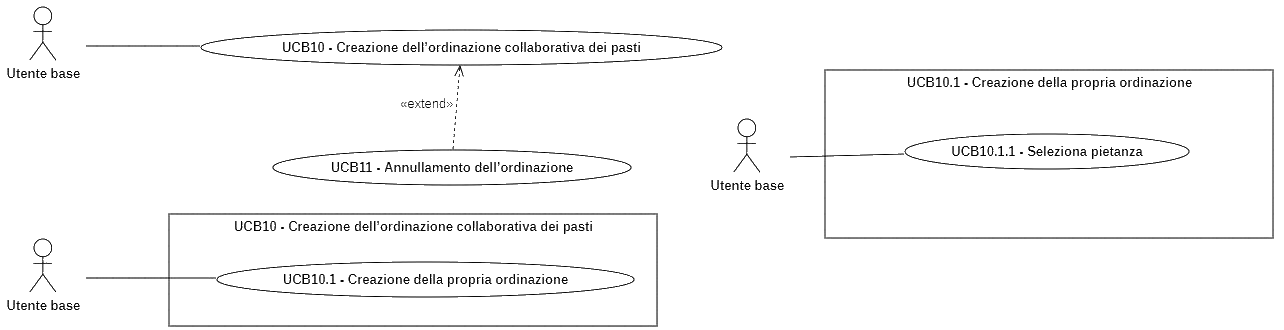
\includegraphics[width=0.99\textwidth]{./uml/UCB10-UCB11.png} 
	\caption{Creazione dell'ordinazione collaborativa dei pasti}
	\label{fig:UCB12-13}
  \end{figure}

\begin{itemize}
	\item \textbf{Attore principale:} Utente base.

	\item \textbf{Precondizioni:}
	      \begin{itemize}
		      \item L'Utente base ha effettuato l'accesso al Sistema (vedi \autoref{usecase:Effettua accesso}).
		      \item L'Utente base ha effettuato una prenotazione (bedi \autoref{usecase:Prenotazione di un tavolo}).
		      \item L'Utente base sta visualizzando la lista delle prenotazioni (vedi \autoref{usecase:Visualizzazione lista delle prenotazioni}), la cui prenotazione si deve trovare nello stato: "Accettata"  (vedi \autoref{usecase:Accetta prenotazione}) o "In attesa".
	      \end{itemize}

	\item \textbf{Postcondizione:} Un Utente base ha ordinato le pietanze per la prenotazione effettuata.

	\item \textbf{Scenario principale:}
	      \begin{enumerate}
		      \item L'Utente base visualizza le ordinazioni di tutti gli altri commensali collegati alla stessa prenotazione;
		      \item L'Utente base crea il proprio ordine$^G$ (vedi \autoref{usecase:Creazione della propria ordinazione});
		      \item L'Utente base modifica il proprio ordine (vedi \autoref{usecase:Modifica della propria ordinazione});

		      \item L'Utente base invia la propria ordinazione;

		      \item Tutti gli Utenti base che partecipano all'ordinazione collaborativa dei pasti devono
		            ivniare la loro ordinazione;
		      \item Il Sistema memorizza l'ordine per ogni utente.
	      \end{enumerate}

	\item \textbf{Scenario secondario:}
	      \begin{itemize}
		      \item L'Utente base annulla l'ordinazione (vedi
		            \autoref{usecase:Annullamento dell'ordinazione}).
		            \begin{enumerate}
			            \item L'Utente base annulla l'ordinazione;
			            \item Il Sistema aggiorna l'ordinazione.
		            \end{enumerate}
	      \end{itemize}
\end{itemize}


\subusecasebase{Creazione della propria ordinazione}
\label{usecase:Creazione della propria ordinazione}
\begin{itemize}
	\item \textbf{Attore principale:} Utente base.

	\item \textbf{Precondizione:} L'Utente base sta effettuando un ordinazione collaborativa dei pasti (vedi \autoref{usecase:Creazione dell'ordinazione collaborativa dei pasti});

	\item \textbf{Postcondizioni:}
	      \begin{itemize}
		      \item L'Utente base ha creato il proprio ordine.
		      \item Il Sistema aggiorna le informazioni inerenti al suo ordine.
	      \end{itemize}

	\item \textbf{Scenario principale:}
	      \begin{enumerate}
		      \item L'Utente base seleziona delle pietanze (vedi \autoref{usecase:Seleziona pietanza});
		      \item L'Utente base conferma il proprio ordine;
		      \item Il Sistema aggiorna il riepilogo dell'ordinazione.
	      \end{enumerate}
\end{itemize}


\subsubusecasebase{Seleziona pietanza}
\label{usecase:Seleziona pietanza}
\begin{itemize}
	\item \textbf{Attore principale:} Utente base.

	\item \textbf{Precondizione:} L'Utente base si trova nella sezione "Creazione della propria ordinazione" (vedi \autoref{usecase:Creazione della propria ordinazione}).

	\item \textbf{Postcondizione:} L'Utente base ha selezionato una pietanza.

	\item \textbf{Scenario principale:}
	      \begin{enumerate}
		      \item L'Utente base seleziona tra le lista delle pietanze una che vuole aggiungere al proprio ordine;
		      \item L'Utente base seleziona la quantità della pietanza;
		      \item L'Utente base conferma la sua selezione;
		      \item Il Sistema registra la sua selezione.
	      \end{enumerate}
\end{itemize}
